\documentclass[11pt]{article}

\usepackage[T1]{fontenc}
\usepackage[utf8]{inputenc}
\usepackage{lmodern}
\usepackage[margin=1in]{geometry}
\usepackage{amsmath}
\usepackage{amssymb}
\usepackage{amsthm}
\usepackage{array}
\usepackage{bbm}
\usepackage{booktabs}
\usepackage[labelfont=bf]{caption}
\usepackage{float}
\usepackage{graphicx}
\usepackage{hyperref}
\usepackage{listings}
\usepackage{longtable}
\usepackage{makecell}
\usepackage{multirow}
\usepackage[round,authoryear]{natbib}
\usepackage{url}
\usepackage{xcolor}

\graphicspath{{build/figures/}}
\hypersetup{
  colorlinks = true,
  linkcolor = blue,
  citecolor = blue,
  urlcolor = blue
}

\setlength{\parindent}{0pt}
\setlength{\parskip}{0.75em}
\allowdisplaybreaks

\lstdefinestyle{rstyle}{
  basicstyle=\ttfamily\small,
  breaklines=true,
  columns=fullflexible,
  frame=single,
  keepspaces=true,
  showstringspaces=false
}
\lstset{style=rstyle, language=R}

\DeclareMathOperator*{\E}{E}
\DeclareMathOperator*{\logit}{logit}
\DeclareMathOperator*{\Bernoulli}{Bernoulli}
\DeclareMathOperator*{\Beta}{Beta}

\newtheorem{proposition}{Proposition}
\newtheorem{lemma}[proposition]{Lemma}

\input{build/generated-values.tex}

\title{Likelihood-ratio tests for continuous outcomes truncated by death}
\author{
  Andreas Kryger Jensen and Theis Lange\\
  Section of Biostatistics, Department of Public Health\\
  University of Copenhagen
}
\date{}

\begin{document}

\maketitle

\begin{abstract}
Patient-reported outcomes, including quality-of-life assessments, are increasingly used as primary or secondary endpoints in randomized clinical trials. These outcomes become challenging to analyze when death, or a similar event, renders the outcome undefined. A common pragmatic solution is to assign such patients the lowest possible score and then compare treatment groups with a standard test on the resulting composite outcome. Although medically interpretable, that analysis can lose substantial power because it does not separate effects on the atom from effects on the continuous part of the distribution. We propose likelihood-ratio tests that retain the clinically meaningful composite outcome while targeting the joint null hypothesis of no treatment effect on either component. We present both a parametric and a semi-parametric version, discuss their large-sample calibration, and illustrate the resulting gain in power in simulations and in a real-data application with a substantively meaningful atom.
\end{abstract}

\begin{center}
\textbf{Keywords:} Quality of Life, Randomized Controlled Trials,\\
Truncated Outcomes, Semi-Continuous Distributions, Empirical Likelihood
\end{center}

\section{Introduction}

Patient-reported outcomes are increasingly used in medical intervention research, including randomized controlled trials (RCTs). Quality-of-life scores are a prominent example. When such outcomes are continuous but skewed or otherwise non-normal, analysts often rely on rank-based procedures such as the Mann--Whitney--Wilcoxon rank-sum test \citep{wilcoxon3001968individual,mann1947test}, which we refer to simply as the Wilcoxon test. That approach works well when the outcome is defined and observed for all participants. In many clinical settings, however, death or a related event makes the outcome undefined for part of the study population. This is common, for example, in intensive-care trials with substantial mortality.

\textbf{[TODO: Add current references documenting the use of rank-based analyses and lowest-score composite encodings for patient-reported outcomes truncated by death.]}

One pragmatic response is to encode death by the lowest possible score and to apply a standard one-dimensional analysis to the resulting composite outcome. This preserves a clinically meaningful ordering, but it creates a statistical difficulty. The composite outcome is no longer purely continuous: it contains both an atom and a continuous component. A rank-based test treats the atom largely through ties and, more importantly, targets a null hypothesis that does not distinguish between effects on survival and effects on the continuous outcome among survivors. As a result, such tests can lose considerable power, especially when treatment affects the two components in different directions.

We therefore model the binary component and the continuous component separately while combining them in a single likelihood-ratio test of no treatment effect on either component. The procedure yields one p-value suitable for a prespecified primary analysis and, unlike a Wilcoxon-type test, it also provides interpretable effect estimates and confidence intervals for the continuous and binary components. To accommodate non-normal outcomes among observed values, we consider both a parametric version and a semi-parametric version based on empirical likelihood.

Although we motivate the method using quality of life truncated by death, the same structure appears whenever one special value has a different scientific meaning than the rest of an otherwise continuous scale. An intensive-care example is days alive and out of hospital within 90 days of randomization, where a value of zero carries qualitatively different information than the positive part of the scale. The same framework also accommodates baseline covariates, so the method is relevant beyond randomized trials.

\textbf{[TODO: Add a short related-work paragraph positioning this method relative to other analyses for truncation by death, composite endpoints, and survivor-only comparisons, and clarify the intended scope of the present approach.]}

The rest of the paper is organized as follows. Section~\ref{sec:method} introduces the statistical setup and the proposed tests. Section~\ref{sec:software-implementation} describes the R implementation. Section~\ref{sec:simulation-study} reports a simulation study, Section~\ref{sec:application} presents a real-data application, and Section~\ref{sec:discussion} concludes. Additional simulation results and a derivation of the empirical-likelihood component are collected in Appendix~\ref{app:supplementary-simulation-results} and Appendix~\ref{app:supplementary-derivation}.

\section{Method}\label{sec:method}

We observe independent and identically distributed random variables $(Y_i, A_i, R_i, X_i)$ for $i = 1, \ldots, n$, where $Y_i$ is a continuous outcome when it is defined, $A_i \in \{0,1\}$ indicates whether the outcome is defined and observed, $R_i \in \{0,1\}$ is the treatment indicator, and $X_i$ is a $p$-dimensional vector of baseline covariates. Because $Y_i$ is only meaningful when $A_i = 1$, the scientific null hypothesis of no treatment effect is
\begin{align*}
  \mathcal{L}(Y_i \mid A_i = 1, R_i = 1, X_i)
  &= \mathcal{L}(Y_i \mid A_i = 1, R_i = 0, X_i),\\
  \Pr(A_i = 1 \mid R_i = 1, X_i)
  &= \Pr(A_i = 1 \mid R_i = 0, X_i).
\end{align*}
In practice, analysts often replace this bivariate object by a single combined outcome
\begin{align}
  \widetilde{Y}_i = Y_i \mathbbm{1}(A_i = 1) + \mathcal{E}\mathbbm{1}(A_i = 0),\label{eq:combinedOutcome}
\end{align}
where $\mathcal{E}$ is a fixed atom representing the undefined outcome. The distribution of $\widetilde{Y}_i$ is therefore a mixture of a point mass at $\mathcal{E}$ and a continuous distribution on the support of $Y_i \mid A_i = 1$.

The conditional mean of the combined outcome is
\begin{align*}
  \E[\widetilde{Y}_i \mid R_i, X_i]
  = \E[Y_i \mid A_i = 1, R_i, X_i]\Pr(A_i = 1 \mid R_i, X_i)
  + \mathcal{E}\Pr(A_i = 0 \mid R_i, X_i).
\end{align*}
This quantity can be identical between treatment groups even when treatment affects both the observation probability and the continuous component. To see this, let
\[
\E[Y_i \mid A_i = 1, R_i = 0, X_i] = \mu(X_i), \qquad
\E[Y_i \mid A_i = 1, R_i = 1, X_i] = \mu(X_i) + \mu_\delta(X_i),
\]
and, for simplicity, set $\mathcal{E} = 0$. Then
\begin{align}
  \Delta(X_i)
  &= \E[\widetilde{Y}_i \mid R_i = 1, X_i] - \E[\widetilde{Y}_i \mid R_i = 0, X_i]\label{eq:Delta}\\
  &= \mu(X_i)\left[\Pr(A_i = 1 \mid R_i = 1, X_i) - \Pr(A_i = 1 \mid R_i = 0, X_i)\right]\nonumber\\
  &\quad + \mu_\delta(X_i)\Pr(A_i = 1 \mid R_i = 1, X_i).\nonumber
\end{align}
Choosing
\[
\mu_\delta(X_i)
= \mu(X_i)\left[\Pr(A_i = 1 \mid R_i = 0, X_i)\Pr(A_i = 1 \mid R_i = 1, X_i)^{-1} - 1\right]
\]
forces $\Delta(X_i)=0$ even though both components depend on treatment. Thus testing $\Delta(X_i)=0$ is generally not equivalent to testing no treatment effect on the joint observed-data structure, and the latter requires two restrictions.

\textbf{[TODO: Add a brief assumptions paragraph here explaining the standing role of the fixed atom $\mathcal{E}$, what substantive events are encoded by $A_i = 0$, and the positivity and identifiability conditions used throughout the inferential development.]}

To exploit that structure, we model the binary and continuous components separately. Let
\begin{align*}
  A_i \mid R_i, X_i &\sim \Bernoulli\left(\pi_i(R_i, X_i)\right),\\
  Y_i \mid A_i = 1, R_i, X_i &\sim F\left(\cdot; \mu_i(R_i, X_i), \Psi\right),
\end{align*}
where $\pi_i(R_i, X_i)$ is the observation probability, $\mu_i(R_i, X_i)$ is a mean parameter for the observed outcomes, and $\Psi$ collects nuisance parameters governing the distribution of the continuous component. If $f(\cdot; \mu_i(R_i, X_i), \Psi)$ denotes the corresponding density, the observed-data likelihood is
\begin{align*}
  L_n(\mu_i(R_i, X_i), \pi_i(R_i, X_i), \Psi)
  = \prod_{i = 1}^n
    f\left(Y_i; \mu_i(R_i, X_i), \Psi\right)^{A_i}
    \pi_i(R_i, X_i)^{A_i}
    \left(1 - \pi_i(R_i, X_i)\right)^{1 - A_i}.
\end{align*}
This factorizes as
\begin{align*}
  L_n(\mu_i(R_i, X_i), \pi_i(R_i, X_i), \Psi)
  = L_{1,n}(\mu_i(R_i, X_i), \Psi)L_{2,n}(\pi_i(R_i, X_i)),
\end{align*}
where
\begin{align*}
  L_{1,n}(\mu_i(R_i, X_i), \Psi)
  &= \prod_{i = 1}^n f\left(Y_i; \mu_i(R_i, X_i), \Psi\right)^{A_i},\\
  L_{2,n}(\pi_i(R_i, X_i))
  &= \prod_{i = 1}^n \pi_i(R_i, X_i)^{A_i}\left(1 - \pi_i(R_i, X_i)\right)^{1 - A_i}.
\end{align*}
The factorization follows from the likelihood construction; it does not require independence between the value of $Y_i$ and the event $A_i = 1$.

We now impose generalized linear models on the two components:
\begin{align}
  \logit \Pr(A_i = 1 \mid R_i, X_i)
  &= \beta_0 + \beta_\delta R_i + s_\beta(X_i),\label{eq:glm1}\\
  \E[Y_i \mid A_i = 1, R_i, X_i]
  &= \mu_0 + \mu_\delta R_i + s_\mu(X_i),\label{eq:glm2}
\end{align}
where $s_\mu$ and $s_\beta$ are finite-dimensional regression terms for the additional covariates. The parameter $\mu_\delta$ is the mean difference among observed outcomes, and $\beta_\delta$ is the log odds-ratio of being observed.

On the original outcome scale, $\mu_\delta$ quantifies how treatment shifts the positive part of the outcome distribution among subjects with observed outcomes, whereas $\beta_\delta$ quantifies how treatment changes the odds that the outcome is observed at all. Reporting the pair therefore separates improvement in the continuous component from improvement in the probability of escaping the atom. This two-component contrast is the scientific target of the proposed likelihood-ratio test. It remains informative even when a single combined-outcome contrast such as $\Delta(X_i)$ is zero because the two components offset each other.

For fixed treatment contrasts $(\mu_\delta,\beta_\delta)$, the profile likelihood-ratio statistic is
\begin{equation}
\label{eq:LRTtotal}
\begin{aligned}
  W_n^P(\mu_\delta, \beta_\delta)
  &= W_{1,n}^P(\mu_\delta) + W_{2,n}^P(\beta_\delta),\\
  W_{1,n}^P(\mu_\delta)
  &= -2\log \frac{\sup\limits_{\mu_0, s_\mu, \Psi} L_{1,n}(\mu_0, \mu_\delta, s_\mu, \Psi)}
  {\sup\limits_{\mu_0, \mu_\delta, s_\mu, \Psi} L_{1,n}(\mu_0, \mu_\delta, s_\mu, \Psi)},\\
  W_{2,n}^P(\beta_\delta)
  &= -2\log \frac{\sup\limits_{\beta_0, s_\beta} L_{2,n}(\beta_0, \beta_\delta, s_\beta)}
  {\sup\limits_{\beta_0, \beta_\delta, s_\beta} L_{2,n}(\beta_0, \beta_\delta, s_\beta)}.
\end{aligned}
\end{equation}
The null hypothesis of no treatment effect is tested with $W_n^P(0,0)$.

\textit{Parametric version.}

In the parametric version, one specifies a parametric model for the observed outcomes. For example, combining Equation~(\ref{eq:glm2}) with a normal model yields
\begin{align*}
  Y_i \mid A_i = 1, R_i, X_i
  \sim N\left(\mu_0 + \mu_\delta R_i + s_\mu(X_i), \sigma^2\right).
\end{align*}
This produces the usual Gaussian likelihood-ratio statistic for $W_{1,n}^P(\mu_\delta)$. Other parametric families can be used in the same way when scientifically appropriate.

\begin{proposition}
Assume that the parametric model for $Y_i \mid A_i = 1, R_i, X_i$ is correctly specified, that the regression models in Equations~(\ref{eq:glm1}) and~(\ref{eq:glm2}) are finite-dimensional and correctly specified, that the true parameter lies in the interior of the parameter space, that the model is identifiable with nonsingular Fisher information, and that $\Pr(A_i = 1 \mid R_i = r, X_i) > 0$ almost surely for $r = 0,1$. Let $m_r = \sum_{i = 1}^n \mathbbm{1}(R_i = r)$ and assume $m_0, m_1 \to \infty$ with $m_1 / m_0 \to c \in (0,\infty)$. Then, under the null hypothesis $\mu_\delta = \beta_\delta = 0$, the profile likelihood-ratio statistic $W_n^P(0,0)$ in Equation~(\ref{eq:LRTtotal}) converges in distribution to $\chi^2_2$.
\end{proposition}

\begin{proof}
Under the stated regularity conditions, the joint likelihood is a regular finite-dimensional likelihood with two scalar restrictions under the null: one in the continuous component and one in the Bernoulli component. Because the likelihood factorizes into $L_{1,n}$ and $L_{2,n}$, the joint likelihood-ratio statistic is exactly the sum of the corresponding component likelihood-ratio statistics. Wilks' theorem \citep{wilks1938large} therefore yields the $\chi^2_2$ limit.
\end{proof}

In practice, this test is easy to compute with standard software: one fits the observed-outcome model with and without the treatment term and does the same for the logistic model for $A_i$, then adds the two log-likelihood differences according to Equation~(\ref{eq:LRTtotal}). At the 5\% level the critical value is $5.99$, and at the 1\% level it is $9.21$.

\textit{Semi-parametric version.}

The parametric test depends on the chosen distributional model for the observed outcomes. To relax that assumption, we replace the first component by a profile empirical likelihood while retaining the Bernoulli likelihood for $A_i$. When there are no additional covariates, the resulting procedure is fully non-parametric for the observed-outcome component.

In the current \texttt{TruncComp2} implementation, the same additive models in Equations~(\ref{eq:glm1}) and~(\ref{eq:glm2}) also support covariate-adjusted semi-parametric fits. The binary component remains the logistic likelihood-ratio statistic for $\beta_\delta$ under the model $\logit \Pr(A_i = 1 \mid R_i, X_i) = \beta_0 + \beta_\delta R_i + s_\beta(X_i)$. The continuous component replaces the no-covariate empirical likelihood by a regression empirical likelihood for the treatment coefficient $\mu_\delta$ in the observed-outcome model $\E[Y_i \mid A_i = 1, R_i, X_i] = \mu_0 + \mu_\delta R_i + s_\mu(X_i)$, profiling over the nuisance regression terms in $s_\mu(X_i)$. The resulting adjusted joint statistic still has the form $W_\mu + W_\alpha$ and is compared with $\chi^2_2$ under regularity. In that adjusted setting the software targets the conditional pair $(\mu_\delta,\beta_\delta)$ rather than a standardized marginal combined-outcome contrast $\Delta$.

To simplify the presentation, we now assume that $X_i$ is absent. Let
\[
\mathcal{I}_0 = \{i = 1,\ldots,n : R_i = 0, A_i = 1\},
\qquad
\mathcal{I}_1 = \{i = 1,\ldots,n : R_i = 1, A_i = 1\}.
\]
Lemma~\ref{lem:empirical-likelihood-derivation} in Appendix~\ref{app:supplementary-derivation} shows that, for fixed $(\mu,\mu_\delta)$, the empirical-likelihood deviance for the observed outcomes is
\begin{align}
  \widetilde{W}_{1,n}(\mu,\mu_\delta)
  &= 2\Biggl(
    \sum_{i \in \mathcal{I}_0}\log\left(1 + \lambda_1(Y_i - \mu)\right)
    + \sum_{j \in \mathcal{I}_1}\log\left(1 + \lambda_2(Y_j - \mu - \mu_\delta)\right)
  \Biggr),\label{eq:nonparametric}
\end{align}
where $\lambda_1$ and $\lambda_2$ solve
\begin{align*}
  \frac{1}{|\mathcal{I}_0|}\sum_{i \in \mathcal{I}_0}
  \frac{Y_i - \mu}{1 + \lambda_1(Y_i - \mu)} &= 0,\\
  \frac{1}{|\mathcal{I}_1|}\sum_{j \in \mathcal{I}_1}
  \frac{Y_j - \mu - \mu_\delta}{1 + \lambda_2(Y_j - \mu - \mu_\delta)} &= 0.
\end{align*}
The profile version is obtained by minimizing over the nuisance mean:
\begin{align*}
  \widetilde{W}_{1,n}^P(\mu_\delta) = \inf_{\mu \in \mathbb{R}} \widetilde{W}_{1,n}(\mu,\mu_\delta).
\end{align*}
The admissible values of $\mu$ are those for which the corresponding constrained means lie in the convex hull of the observed outcomes in each group.

For interior feasible means, the dual parameters $\lambda_1$ and $\lambda_2$ are determined by one-dimensional root equations with unique roots on their admissible intervals. The implementation therefore solves each dual equation by scalar root-finding, evaluating slightly inside the feasibility bounds to avoid numerical instability when the constrained mean approaches the convex-hull boundary. The profiled nuisance mean is obtained by root-finding on the profile gradient when that gradient changes sign across the feasible interval and otherwise by direct one-dimensional optimization over the feasible set. If a candidate constraint falls outside the feasible range or effectively collapses onto the convex-hull boundary, the corresponding empirical-likelihood statistic is treated as infinite rather than extrapolated.

The semi-parametric test statistic is then
\begin{equation}
  \widetilde{W}_n^P(\mu_\delta, \beta_\delta)
  = \widetilde{W}_{1,n}^P(\mu_\delta) + W_{2,n}^P(\beta_\delta).\label{eq:LRT_SP_total}
\end{equation}

\begin{proposition}
Assume that there are no additional covariates, that $\Pr(A_i = 1 \mid R_i = r) > 0$ for $r = 0,1$, and that $m_0, m_1 \to \infty$ with $m_1 / m_0 \to c \in (0,\infty)$. Suppose further that the Bernoulli model for $A_i$ is correctly specified, that under the null hypothesis the observed outcomes in the two treatment groups have a common finite mean, strictly positive finite variance, and support whose convex hull contains that mean as an interior point. Then, under $\mu_\delta = \beta_\delta = 0$, the semi-parametric statistic $\widetilde{W}_n^P(0,0)$ in Equation~(\ref{eq:LRT_SP_total}) converges in distribution to $\chi^2_2$.
\end{proposition}

\begin{proof}
Under the stated conditions, $W_{2,n}^P(0)$ is the usual one-parameter Bernoulli likelihood-ratio statistic, so Wilks' theorem gives a $\chi^2_1$ limit. For the observed outcomes, standard two-sample empirical-likelihood theory for a mean-difference constraint implies that $\widetilde{W}_{1,n}^P(0)$ has the Wilks-type $\chi^2_1$ limit; see \citet{owen1991empirical}. The joint criterion is the sum of these two orthogonal components, so the overall null statistic has the $\chi^2_2$ limit.
\end{proof}

Confidence regions follow by inverting the corresponding likelihood-ratio statistic. For the parametric procedure, an asymptotic $(1-\alpha)100\%$ simultaneous confidence region for $(\mu_\delta,\beta_\delta)$ is
\begin{align*}
  \mathrm{CI}^{(\mu_\delta,\beta_\delta)}_{1-\alpha}
  = \left\{(m,b) \in \mathbb{R}^2 : W_n^P(m,b) \leq \chi^2_2(1-\alpha)\right\}.
\end{align*}
For the semi-parametric procedure, one replaces $W_n^P$ by $\widetilde{W}_n^P$. Correspondingly, the marginal intervals are
\begin{align*}
  \mathrm{CI}^{\mu_\delta}_{1-\alpha}
  &= \left\{m \in \mathbb{R} : W_{1,n}^P(m) \leq \chi^2_1(1-\alpha)\right\}
  \quad \text{or} \quad
  \left\{m \in \mathbb{R} : \widetilde{W}_{1,n}^P(m) \leq \chi^2_1(1-\alpha)\right\},\\
  \mathrm{CI}^{\beta_\delta}_{1-\alpha}
  &= \left\{b \in \mathbb{R} : W_{2,n}^P(b) \leq \chi^2_1(1-\alpha)\right\}.
\end{align*}
We recommend reporting the simultaneous confidence region because it displays the joint uncertainty about the effect on the continuous and binary components.

For successful unadjusted fits, the software also reports several summaries on the combined-outcome scale $\Delta$. The interval \texttt{DeltaMarginalCI} is a descriptive Welch interval for the raw combined-outcome mean difference, \texttt{DeltaProfileCI} is the one-dimensional likelihood-based interval obtained by profiling in $\Delta$, and \texttt{DeltaProjectedCI} is the projection of the full two-dimensional simultaneous region onto the $\Delta$ scale. The projected interval is typically wider because it inherits the full simultaneous statement for $(\mu_\delta,\beta_\delta)$. In a trial report we therefore recommend presenting the joint p-value and the simultaneous region whenever the scientific claim concerns no treatment effect on either component, while using marginal component intervals and any $\Delta$-scale intervals as supporting summaries rather than as substitutes for the joint region.

\section{Software implementation}\label{sec:software-implementation}

We implemented both the parametric and semi-parametric procedures, together with their current software extensions, in the R package \texttt{TruncComp2}, which is available from GitHub \citep{TruncCompGitHub}. We illustrate the interface with the packaged example data set.

The example data set is loaded by

\begin{lstlisting}
library(TruncComp2)
example_data <- loadTruncComp2Example()
\end{lstlisting}

It contains the outcome $Y$ and a binary treatment indicator $R$, with 25 observations in each treatment group. Truncated observations are encoded by the atom $\mathcal{E} = 0$. Figure~\ref{fig:dataExampleHistogram} displays histograms of the outcome in the two groups.

\begin{figure}[htbp]
\centering
\includegraphics[width=0.7\textwidth]{example-histogram.pdf}
\caption{Histograms of the example outcome by treatment group. The atom at zero represents the special outcome value $\mathcal{E} = 0$.}
\label{fig:dataExampleHistogram}
\end{figure}

In this example, the difference in sample means of the combined outcome is \ExampleDelta{}, while a two-sample t-test and a Wilcoxon rank-sum test yield p-values \ExampleTTestP{} and \ExampleWilcoxP{}, respectively. The semi-parametric likelihood-ratio analysis is obtained as follows:

\begin{lstlisting}
fit_splrt <- truncComp(Y ~ R, atom = 0, data = example_data, method = "SPLRT")
fit_lrt <- truncComp(Y ~ R, atom = 0, data = example_data, method = "LRT")
summary(fit_splrt)
summary(fit_lrt)
\end{lstlisting}

In practice, \texttt{LRT} is appropriate when a parametric model for the positive outcomes is scientifically credible and efficiency is the priority, whereas \texttt{SPLRT} is preferable when robustness to non-normal positive outcomes matters more than that distributional assumption.

The output reports estimates of the mean difference among observed outcomes, $\mu_\delta$, and the odds ratio $\exp(\beta_\delta)$ of being observed. It also reports marginal 95\% confidence intervals for the two components, together with the joint likelihood-ratio statistic and its p-value for the null hypothesis of no treatment effect. For successful unadjusted fits from either method, \texttt{confint(..., parameter = c("muDelta", "alphaDelta"))} returns the stored component intervals, \texttt{confint(..., parameter = "Delta", method = "profile")} returns the one-dimensional profile interval for $\Delta$, \texttt{confint(..., parameter = "Delta", method = "projected")} returns the projected interval from the full joint region, and \texttt{confint(..., parameter = "joint")} or \texttt{jointContrastCI(fit)} evaluates the two-dimensional simultaneous region for $(\mu_\delta,\beta_\delta)$, typically visualized on the $(\mu_\delta,\log \text{OR})$ scale. Because the projected \texttt{Delta} interval inherits the full simultaneous statement, it is usually more conservative than the one-dimensional profile interval.

For this data set, both the parametric and semi-parametric analyses reject the joint null hypothesis, in contrast to both the t-test and the Wilcoxon test. The estimated effect is driven primarily by a higher mean among the observed outcomes in the treatment group $R = 1$.

Confidence intervals and the simultaneous confidence region can be extracted with

\begin{lstlisting}
confint(fit_splrt, parameter = c("muDelta", "alphaDelta"))
confint(fit_splrt, parameter = "Delta", method = "profile")
confint(fit_splrt, parameter = "Delta", method = "projected")
confint(fit_splrt, parameter = "joint", plot = TRUE, offset = 1.4, resolution = 50)
jointContrastCI(fit_splrt, plot = FALSE)
\end{lstlisting}

where \texttt{resolution} is the number of grid points used to evaluate the likelihood surface. Figure~\ref{fig:simultConfidence} shows the resulting surface and the 95\% simultaneous confidence region. The origin $(0,0)$ lies well outside the region, which matches the strong rejection of the joint null.

Current package functionality extends beyond the no-covariate presentation in Section~\ref{sec:method}. Both methods accept additive baseline adjustment through \texttt{adjust = \textasciitilde{} ...}, and \texttt{TruncComp2} ships a second packaged example through \texttt{loadTruncComp2AdjustedExample()}. In adjusted fits, the reported \texttt{muDelta} and \texttt{alphaDelta} are conditional treatment effects from the observed-outcome and logistic submodels, so the software intentionally leaves \texttt{Delta} undefined. The adjusted interface therefore supports only marginal component intervals; simultaneous regions and $\Delta$-based intervals are not currently implemented there. The companion default interface \texttt{truncComp.default(y, a, r, ..., atom = NULL)} can also infer the atom automatically when all observations with \texttt{a = 0} share the same finite value. For synthetic examples and checks, \texttt{simulateTruncatedData()} generates the canonical two-group data structure used throughout the package.

An adjusted analysis is obtained through the same front end:

\begin{lstlisting}
adjusted_data <- loadTruncComp2AdjustedExample()
fit_adjusted <- truncComp(Y ~ R, atom = 0, data = adjusted_data,
                          method = "SPLRT", adjust = ~ L)
confint(fit_adjusted, parameter = c("muDelta", "alphaDelta"))
\end{lstlisting}

In the packaged adjusted example, both methods attenuate after adjustment, which illustrates how the conditional treatment effects can differ materially from the unadjusted component contrasts.

\begin{figure}[htbp]
\centering
\includegraphics[width=0.62\textwidth]{example-simultaneous-confidence.pdf}
\caption{Simultaneous semi-parametric likelihood-ratio surface for $(\mu_\delta,\beta_\delta)$ in the example data.}
\label{fig:simultConfidence}
\end{figure}

\section{Simulation study}\label{sec:simulation-study}

We investigated power and null calibration in six simulation scenarios. Throughout, treatment was randomized one-to-one between two groups, the atom was fixed at $\mathcal{E} = 0$, and the combined outcome was therefore $\widetilde{Y}_i = A_iY_i$.

Table~\ref{tab:simulation} lists the data-generating mechanisms. The scenarios were chosen to isolate the practically important comparisons. Scenario~1 is a low-atom normal reference case, Scenario~2 isolates a pure atom-probability effect, Scenario~3 forces the atom and continuous components to move in opposite directions while keeping the combined-outcome mean fixed, Scenario~4 makes both components move in the same direction, Scenario~5 introduces a gamma shape change together with a survivor-mean shift, and Scenario~6 uses rare extreme outliers to create a Wilcoxon-favorable regime.

\begin{table}[!h]
\centering
\caption{\label{tab:simulation}Simulation scenarios S1--S6 for effect levels $h=0,1,2,3$}
\centering
\resizebox{\ifdim\width>\linewidth\linewidth\else\width\fi}{!}{
\begin{tabular}[t]{llll}
\toprule
Scenario & Configuration & \makecell[l]{Probability outside atom\\ $\pi_{r,h}=\Prob(A=1\mid R=r)$} & \makecell[l]{Non-atom law\\ $F_{r,h}^c$}\\
\midrule
S1 & \makecell[l]{Normal non-atom shift,\\ low atom probability} & \makecell[l]{$\pi_{0,h} = \pi_{1,h} = 0.85$} & \makecell[l]{$F_{0,h}^c = N(3, 1)$\\ $F_{1,h}^c = N(3 + \delta_h, 1)$\\ $(\delta_0,\ldots,\delta_3) = (0, 0.20, 0.35, 0.50)$}\\
S2 & \makecell[l]{Effect only on probability\\ outside atom} & \makecell[l]{$\pi_{0,h} = 0.45$\\ $(\pi_{1,0},\ldots,\pi_{1,3}) = (0.45, 0.50, 0.55, 0.60)$} & \makecell[l]{$F_{0,h}^c = F_{1,h}^c = N(3, 1)$}\\
S3 & \makecell[l]{Antagonistic\\ cancellation} & \makecell[l]{$\pi_{0,h} = 0.50$\\ $(\pi_{1,0},\ldots,\pi_{1,3}) = (0.50, 0.525, 0.55, 0.60)$} & \makecell[l]{$F_{0,h}^c = N(3, 1)$\\ $F_{1,h}^c = N(1.5 / \pi_{1,h}, 1)$}\\
S4 & \makecell[l]{Concordant joint\\ improvement} & \makecell[l]{$\pi_{0,h} = 0.50$\\ $(\pi_{1,0},\ldots,\pi_{1,3}) = (0.50, 0.55, 0.60, 0.65)$} & \makecell[l]{$F_{0,h}^c = N(3, 1)$\\ $F_{1,h}^c = N(3 + 0.15h, 1)$}\\
S5 & \makecell[l]{Gamma shape change\\ with mean shift} & \makecell[l]{$\pi_{0,h} = \pi_{1,h} = 0.65$} & \makecell[l]{$F_{0,h}^c = \Gamma(9, 3/9)$\\ $F_{1,h}^c = \Gamma(k_h, m_h / k_h)$\\ $(k_0,\ldots,k_3) = (9, 6, 4, 2.5)$\\ $(m_0,\ldots,m_3) = (3.0, 3.2, 3.4, 3.6)$}\\
S6 & \makecell[l]{Rare outlier\\ contamination} & \makecell[l]{$\pi_{0,h} = \pi_{1,h} = 0.80$} & \makecell[l]{$F_{r,h}^c = 0.95 N(3 + r\delta_h, 0.35^2)$\\ $\hspace{2.6em}{}+ 0.05 N(10 + r\delta_h, 0.5^2)$\\ $(\delta_0,\ldots,\delta_3) = (0, 0.15, 0.25, 0.35)$}\\
\bottomrule
\end{tabular}}
\end{table}


For each scenario we considered effect levels $h \in \{0, 1, 2, 3\}$, with $h = 0$ as the null configuration, and sample sizes from $50$ to $500$ observations per group in increments of $50$. Every scenario-effect-sample-size cell used 10,000 Monte Carlo repetitions. Power and empirical size were estimated as rejection proportions at the 5\% level, and the worst-case Monte Carlo standard error of an estimated rejection rate was therefore approximately $0.005$. We compared the parametric and semi-parametric likelihood-ratio tests with Welch's two-sample $t$-test and the Wilcoxon rank-sum test applied directly to the combined outcome.

Figure~\ref{fig:powerCurves} shows power as a function of sample size at the strongest non-null level for the four scenarios that most sharply separate the methods: the survival-only case (Scenario~2), the antagonistic cancellation case (Scenario~3), the gamma misspecification case (Scenario~5), and the rare-outlier contamination case (Scenario~6). Figure~\ref{fig:powerEffectCurves} complements that display by plotting power as a function of the effect level at $n = 250$ observations per group for the same four scenarios. The supplementary material reports the corresponding power curves for Scenarios~1 and~4, the full scenario-specific power tables for all $240$ cells, and the null-calibration displays for the $h = 0$ settings.

\begin{figure}[htbp]
\centering
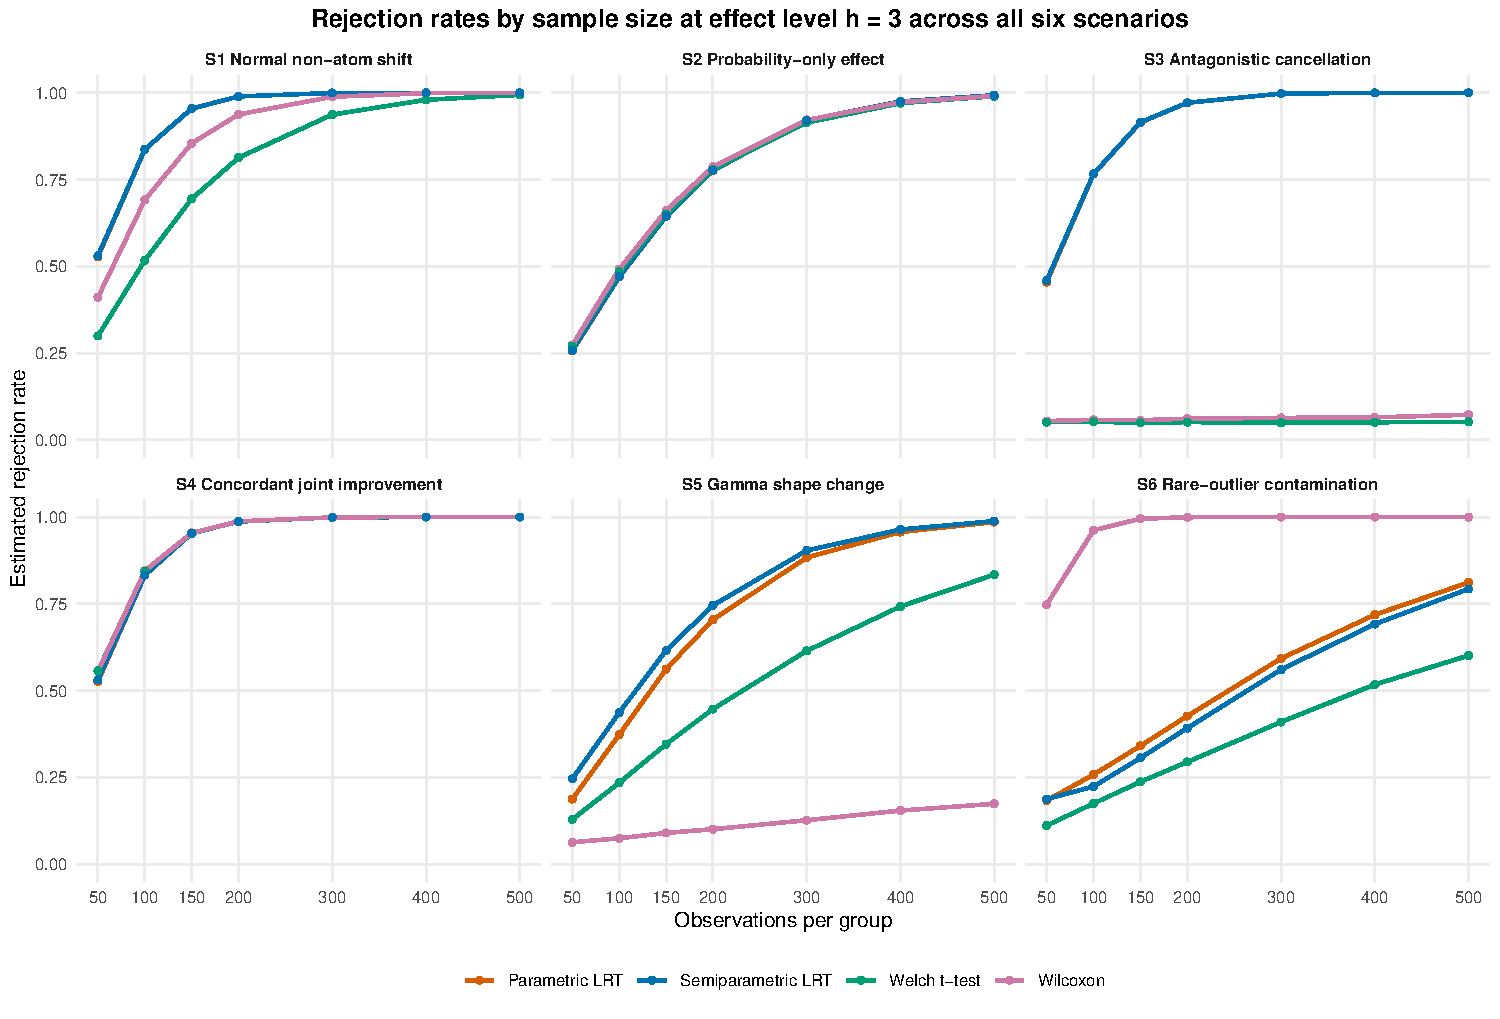
\includegraphics[width=0.84\textwidth]{power-curves.pdf}
\caption{Estimated power as a function of sample size at the strongest non-null level for Scenarios~2, 3, 5, and 6.}
\label{fig:powerCurves}
\end{figure}

\begin{figure}[htbp]
\centering
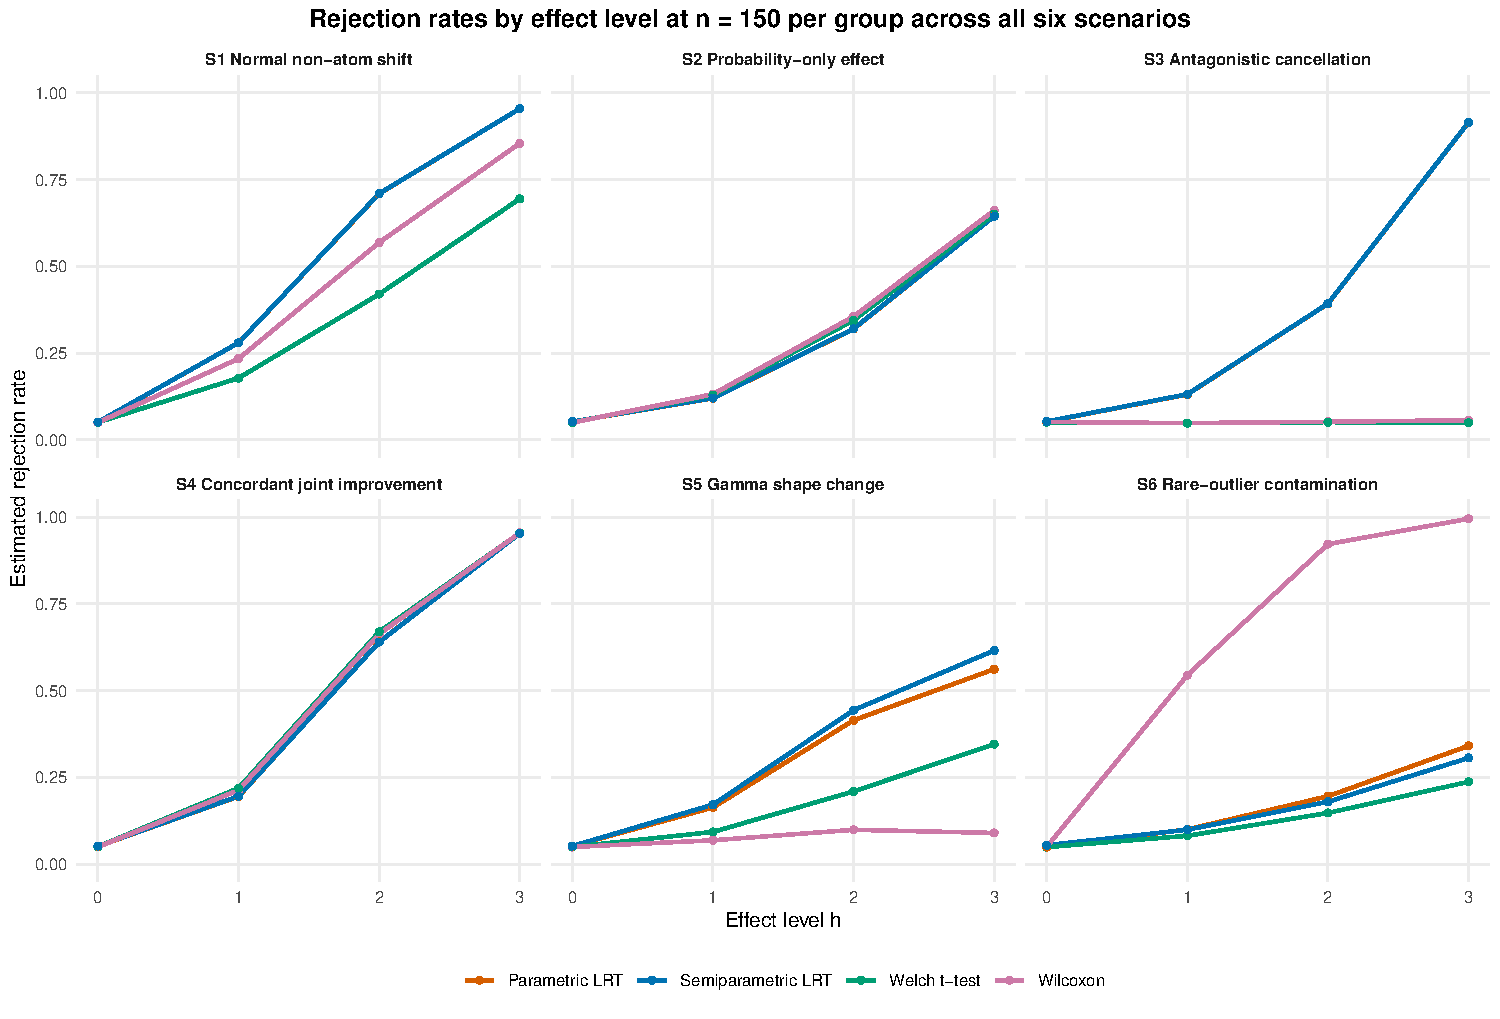
\includegraphics[width=0.84\textwidth]{power-effects.pdf}
\caption{Estimated power as a function of effect level at $n = 250$ observations per group for Scenarios~2, 3, 5, and 6.}
\label{fig:powerEffectCurves}
\end{figure}

\section{Application}\label{sec:application}

To illustrate the same continuous-plus-atom structure in a different applied setting, the current manuscript build pipeline uses \ApplicationDatasetDescription{} ($n = \ApplicationN{}$). Here the outcome is \ApplicationOutcomeLabel{}, and the atom at zero corresponds to \ApplicationAtomMeaning{}. This is not a truncation-by-death example, but it has the same statistical form of a point mass at a substantively distinct atom together with a continuous positive part.

Figure~\ref{fig:application} shows the empirical distributions in the two treatment groups together with the simultaneous confidence region for the semi-parametric analysis. In our notation, we code $A = 0$ when the outcome equals zero and $A = 1$ otherwise; $Y$ then denotes the positive part of the outcome among subjects with $A = 1$.

\begin{figure}[htbp]
\centering

\includegraphics[width=\textwidth]{application.pdf}
\caption{\ApplicationDatasetName{}: histograms of \ApplicationOutcomeShort{} by treatment group (left and middle panels) and the semi-parametric simultaneous confidence region for $(\mu_\delta,\beta_\delta)$ (right panel).}
\label{fig:application}
\end{figure}

For this application, the Wilcoxon test yields p-value \ApplicationWilcoxP{}, which does not cross the prespecified 5\% threshold. The parametric likelihood-ratio test yields p-value \ApplicationLRTP{}, and the semi-parametric analysis yields p-value \ApplicationSPLRTP{}.

At the 5\% level, \ApplicationConclusionSummary{}

The simultaneous confidence region in Figure~\ref{fig:application} suggests that the dominant treatment signal lies in the continuous component rather than in the probability of the atom. In this application, \ApplicationComponentSummary{}

\section{Discussion}\label{sec:discussion}

We have presented parametric and semi-parametric likelihood-ratio tests for continuous outcomes that contain a clinically meaningful atom, such as outcomes truncated by death. The key idea is to retain the composite outcome used in practice while testing a null hypothesis that separates the binary and continuous components. This produces a single p-value, together with interpretable component-wise effect estimates and confidence intervals.

The simulations and the application example show why this distinction matters. Rank-based analyses can perform well when treatment acts primarily through one dimension of the combined outcome, but they can lose substantial power when the atom and the continuous part move in different directions or when the continuous component has a shape that is poorly summarized by ranks. In contrast, the proposed likelihood-ratio framework matches the scientific structure of the problem more directly.

This is particularly useful when an RCT requires a single prespecified primary analysis for an outcome that combines survival with a continuous measurement. The parametric version is straightforward to compute when a plausible model for the observed outcomes is available, whereas the semi-parametric version avoids that distributional commitment. Both procedures are asymptotic, however, so they require adequate numbers of observed outcomes in each treatment group for the large-sample calibration to be reliable.

Several limitations should be kept in mind. First, the calibration is asymptotic, so small samples or very sparse positive outcomes can make both the parametric and semi-parametric approximations unreliable. Second, the parametric procedure inherits the usual risk of model misspecification for the positive part of the outcome, while the adjusted semi-parametric procedure still requires a regular logistic fit and enough observed outcomes relative to the adjusted design matrix. In the current \texttt{TruncComp2} implementation, adjusted fits return clean failure rather than approximate fallback behavior when separation, rank deficiency, or infeasible empirical-likelihood constraints arise. Finally, the two-component target $(\mu_\delta,\beta_\delta)$ is not the same estimand as approaches based on principal stratification, survivor-average causal effects, or other standardized marginal truncation-by-death contrasts, so the method should be interpreted as targeting the joint observed-data structure rather than those alternative causal summaries.

\clearpage
\appendix
\section{Supplementary simulation results}\label{app:supplementary-simulation-results}

This appendix collects the simulation figures and tables referenced in Section~\ref{sec:simulation-study}. Figure~\ref{fig:suppPowerCurves} shows the sample-size power curves for the remaining two scenarios from the main design, and Figure~\ref{fig:type1Curves} summarizes the $h = 0$ null-calibration results across all six scenarios.

\begin{figure}[htbp]
\centering
\includegraphics[width=0.84\textwidth]{supplementary-power-curves.pdf}
\caption{Estimated power as a function of sample size at the strongest non-null level for Scenarios~1 and~4.}
\label{fig:suppPowerCurves}
\end{figure}

\begin{figure}[htbp]
\centering
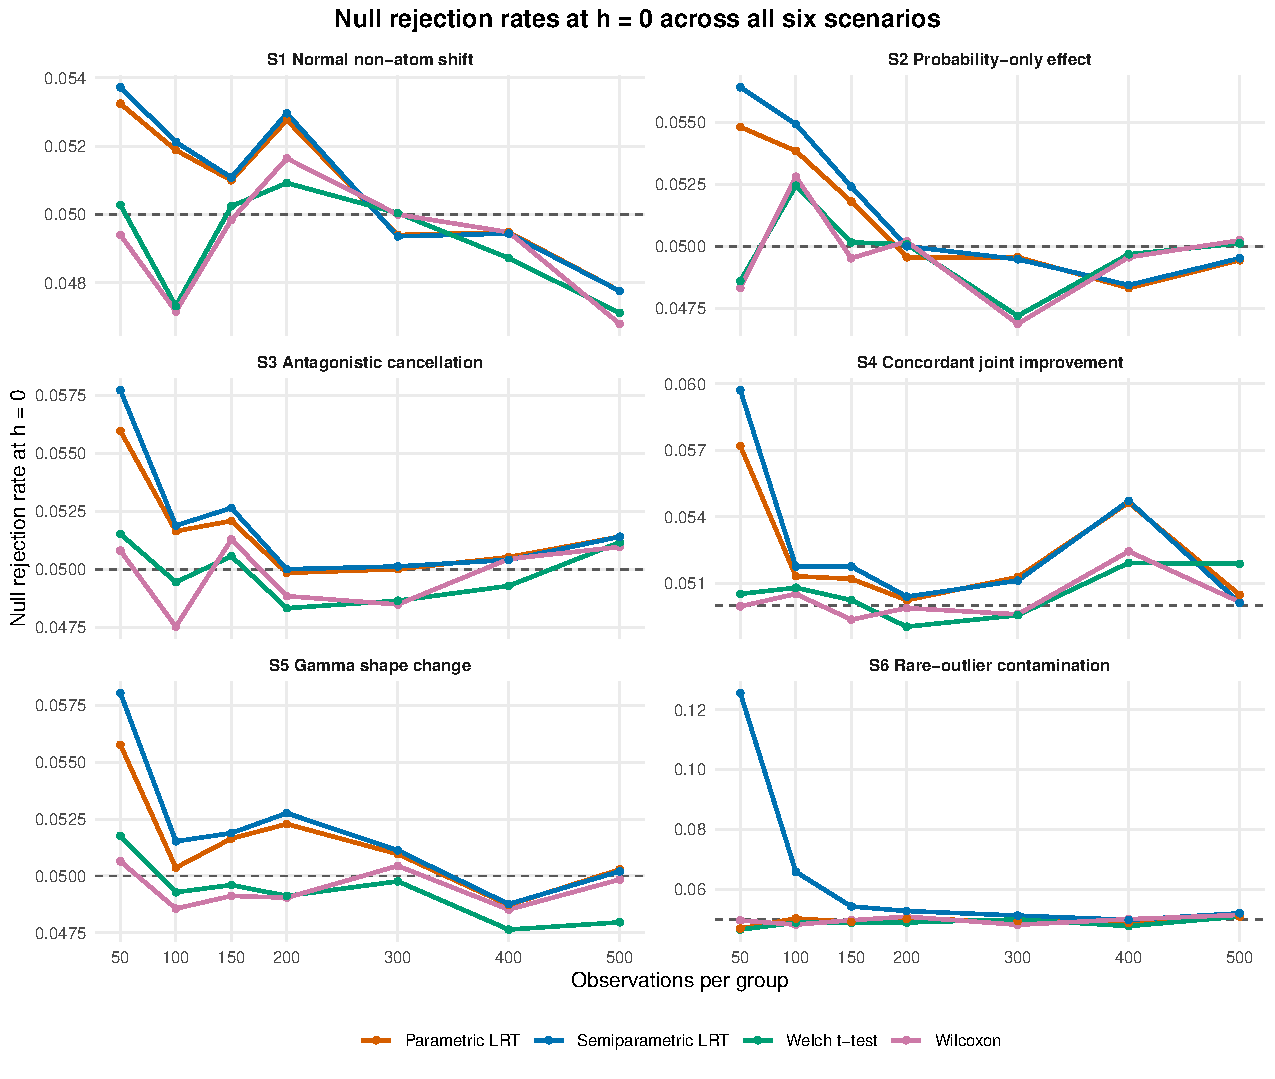
\includegraphics[width=0.84\textwidth]{type1-curves.pdf}
\caption{Empirical size at effect level $h = 0$ across all six simulation scenarios. The dashed line marks 0.05 and the dotted lines mark 0.04 and 0.06.}
\label{fig:type1Curves}
\end{figure}

\begingroup\fontsize{7}{9}\selectfont

\begin{longtable}[t]{rrlrrrrr}
\caption{Scenario S1 (Normal non-atom shift, low atom probability): estimated rejection percentages by sample size and effect level}\\
\toprule
$n_{\mathrm{arm}}$ & $h$ & Effect & Expected $\Delta^{(0)}$ & Wilcoxon (\%) & Welch $t$-test (\%) & LRT (\%) & SPLRT (\%)\\
\midrule
\endfirsthead
\caption[]{Scenario S1 (Normal non-atom shift, low atom probability): estimated rejection percentages by sample size and effect level \textit{(continued)}}\\
\toprule
$n_{\mathrm{arm}}$ & $h$ & Effect & Expected $\Delta^{(0)}$ & Wilcoxon (\%) & Welch $t$-test (\%) & LRT (\%) & SPLRT (\%)\\
\midrule
\endhead

\endfoot
\bottomrule
\endlastfoot
50 & 0 & \makecell[l]{$\delta_h = 0.00$} & 0.000 & 4.94 & 5.03 & 5.32 & 5.37\\
100 & 0 & \makecell[l]{$\delta_h = 0.00$} & 0.000 & 4.72 & 4.73 & 5.19 & 5.21\\
150 & 0 & \makecell[l]{$\delta_h = 0.00$} & 0.000 & 4.98 & 5.02 & 5.10 & 5.11\\
200 & 0 & \makecell[l]{$\delta_h = 0.00$} & 0.000 & 5.16 & 5.09 & 5.28 & 5.30\\
300 & 0 & \makecell[l]{$\delta_h = 0.00$} & 0.000 & 5.00 & 5.00 & 4.94 & 4.94\\
400 & 0 & \makecell[l]{$\delta_h = 0.00$} & 0.000 & 4.95 & 4.87 & 4.95 & 4.94\\
500 & 0 & \makecell[l]{$\delta_h = 0.00$} & 0.000 & 4.68 & 4.71 & 4.78 & 4.78\\
50 & 1 & \makecell[l]{$\delta_h = 0.20$} & 0.170 & 10.65 & 9.25 & 12.44 & 12.56\\
100 & 1 & \makecell[l]{$\delta_h = 0.20$} & 0.170 & 16.89 & 13.26 & 20.16 & 20.17\\
150 & 1 & \makecell[l]{$\delta_h = 0.20$} & 0.170 & 23.37 & 17.78 & 27.97 & 27.97\\
200 & 1 & \makecell[l]{$\delta_h = 0.20$} & 0.170 & 29.32 & 21.86 & 35.98 & 36.01\\
300 & 1 & \makecell[l]{$\delta_h = 0.20$} & 0.170 & 40.84 & 30.20 & 50.76 & 50.78\\
400 & 1 & \makecell[l]{$\delta_h = 0.20$} & 0.170 & 52.36 & 39.04 & 64.54 & 64.60\\
500 & 1 & \makecell[l]{$\delta_h = 0.20$} & 0.170 & 60.72 & 45.90 & 74.45 & 74.40\\
50 & 2 & \makecell[l]{$\delta_h = 0.35$} & 0.298 & 22.98 & 17.55 & 28.78 & 29.02\\
100 & 2 & \makecell[l]{$\delta_h = 0.35$} & 0.298 & 41.03 & 30.20 & 51.88 & 52.00\\
150 & 2 & \makecell[l]{$\delta_h = 0.35$} & 0.298 & 56.84 & 41.98 & 70.91 & 70.96\\
200 & 2 & \makecell[l]{$\delta_h = 0.35$} & 0.298 & 69.77 & 53.36 & 83.26 & 83.22\\
300 & 2 & \makecell[l]{$\delta_h = 0.35$} & 0.298 & 85.27 & 69.76 & 95.02 & 95.03\\
400 & 2 & \makecell[l]{$\delta_h = 0.35$} & 0.298 & 93.56 & 81.58 & 98.80 & 98.80\\
500 & 2 & \makecell[l]{$\delta_h = 0.35$} & 0.298 & 97.37 & 89.66 & 99.76 & 99.76\\
50 & 3 & \makecell[l]{$\delta_h = 0.50$} & 0.425 & 41.04 & 29.95 & 52.75 & 53.05\\
100 & 3 & \makecell[l]{$\delta_h = 0.50$} & 0.425 & 69.14 & 51.71 & 83.67 & 83.70\\
150 & 3 & \makecell[l]{$\delta_h = 0.50$} & 0.425 & 85.45 & 69.44 & 95.45 & 95.44\\
200 & 3 & \makecell[l]{$\delta_h = 0.50$} & 0.425 & 93.76 & 81.30 & 98.95 & 98.95\\
300 & 3 & \makecell[l]{$\delta_h = 0.50$} & 0.425 & 98.86 & 93.72 & 99.94 & 99.94\\
400 & 3 & \makecell[l]{$\delta_h = 0.50$} & 0.425 & 99.88 & 97.97 & 100.00 & 100.00\\
500 & 3 & \makecell[l]{$\delta_h = 0.50$} & 0.425 & 99.98 & 99.40 & 100.00 & 100.00\\*
\end{longtable}
\endgroup{}

\begingroup\fontsize{7}{9}\selectfont

\begin{longtable}[t]{rrlrrrrr}
\caption{Scenario S2 (effect only on probability outside atom): estimated rejection percentages by sample size and effect level}\\
\toprule
$n_{\mathrm{arm}}$ & $h$ & Effect & Expected $\Delta^{(0)}$ & Wilcoxon (\%) & Welch $t$-test (\%) & LRT (\%) & SPLRT (\%)\\
\midrule
\endfirsthead
\caption[]{Scenario S2 (effect only on probability outside atom): estimated rejection percentages by sample size and effect level \textit{(continued)}}\\
\toprule
$n_{\mathrm{arm}}$ & $h$ & Effect & Expected $\Delta^{(0)}$ & Wilcoxon (\%) & Welch $t$-test (\%) & LRT (\%) & SPLRT (\%)\\
\midrule
\endhead

\endfoot
\bottomrule
\endlastfoot
50 & 0 & \makecell[l]{$\pi_{1,h} = 0.45$} & 0.00 & 4.83 & 4.86 & 5.48 & 5.64\\
100 & 0 & \makecell[l]{$\pi_{1,h} = 0.45$} & 0.00 & 5.28 & 5.24 & 5.38 & 5.49\\
150 & 0 & \makecell[l]{$\pi_{1,h} = 0.45$} & 0.00 & 4.95 & 5.02 & 5.18 & 5.24\\
200 & 0 & \makecell[l]{$\pi_{1,h} = 0.45$} & 0.00 & 5.02 & 5.01 & 4.96 & 5.00\\
300 & 0 & \makecell[l]{$\pi_{1,h} = 0.45$} & 0.00 & 4.69 & 4.72 & 4.96 & 4.95\\
400 & 0 & \makecell[l]{$\pi_{1,h} = 0.45$} & 0.00 & 4.96 & 4.97 & 4.83 & 4.84\\
500 & 0 & \makecell[l]{$\pi_{1,h} = 0.45$} & 0.00 & 5.02 & 5.01 & 4.94 & 4.95\\
50 & 1 & \makecell[l]{$\pi_{1,h} = 0.50$} & 0.15 & 7.70 & 7.74 & 7.74 & 7.91\\
100 & 1 & \makecell[l]{$\pi_{1,h} = 0.50$} & 0.15 & 9.90 & 9.76 & 9.04 & 9.04\\
150 & 1 & \makecell[l]{$\pi_{1,h} = 0.50$} & 0.15 & 13.13 & 12.89 & 11.96 & 12.01\\
200 & 1 & \makecell[l]{$\pi_{1,h} = 0.50$} & 0.15 & 15.28 & 14.79 & 13.08 & 13.09\\
300 & 1 & \makecell[l]{$\pi_{1,h} = 0.50$} & 0.15 & 20.23 & 19.51 & 17.86 & 17.88\\
400 & 1 & \makecell[l]{$\pi_{1,h} = 0.50$} & 0.15 & 26.26 & 25.10 & 22.88 & 22.90\\
500 & 1 & \makecell[l]{$\pi_{1,h} = 0.50$} & 0.15 & 31.61 & 30.40 & 27.64 & 27.64\\
50 & 2 & \makecell[l]{$\pi_{1,h} = 0.55$} & 0.30 & 14.73 & 14.51 & 13.93 & 14.15\\
100 & 2 & \makecell[l]{$\pi_{1,h} = 0.55$} & 0.30 & 25.27 & 24.69 & 23.11 & 23.11\\
150 & 2 & \makecell[l]{$\pi_{1,h} = 0.55$} & 0.30 & 35.54 & 34.42 & 31.94 & 31.98\\
200 & 2 & \makecell[l]{$\pi_{1,h} = 0.55$} & 0.30 & 45.40 & 43.97 & 41.52 & 41.54\\
300 & 2 & \makecell[l]{$\pi_{1,h} = 0.55$} & 0.30 & 61.90 & 60.21 & 58.91 & 58.90\\
400 & 2 & \makecell[l]{$\pi_{1,h} = 0.55$} & 0.30 & 74.22 & 72.58 & 71.88 & 71.86\\
500 & 2 & \makecell[l]{$\pi_{1,h} = 0.55$} & 0.30 & 83.02 & 81.57 & 81.38 & 81.39\\
50 & 3 & \makecell[l]{$\pi_{1,h} = 0.60$} & 0.45 & 27.30 & 27.02 & 25.59 & 25.84\\
100 & 3 & \makecell[l]{$\pi_{1,h} = 0.60$} & 0.45 & 49.18 & 48.44 & 46.92 & 47.00\\
150 & 3 & \makecell[l]{$\pi_{1,h} = 0.60$} & 0.45 & 66.08 & 64.98 & 64.40 & 64.39\\
200 & 3 & \makecell[l]{$\pi_{1,h} = 0.60$} & 0.45 & 78.67 & 77.90 & 77.57 & 77.59\\
300 & 3 & \makecell[l]{$\pi_{1,h} = 0.60$} & 0.45 & 92.17 & 91.39 & 92.10 & 92.10\\
400 & 3 & \makecell[l]{$\pi_{1,h} = 0.60$} & 0.45 & 97.29 & 97.01 & 97.50 & 97.50\\
500 & 3 & \makecell[l]{$\pi_{1,h} = 0.60$} & 0.45 & 99.09 & 99.00 & 99.30 & 99.30\\*
\end{longtable}
\endgroup{}

\begingroup\fontsize{7}{9}\selectfont

\begin{longtable}[t]{rrlrrrrr}
\caption{Scenario S3 (antagonistic cancellation): estimated rejection percentages by sample size and effect level}\\
\toprule
$n_{\mathrm{arm}}$ & $h$ & Effect & Expected $\Delta^{(0)}$ & Wilcoxon (\%) & Welch $t$-test (\%) & LRT (\%) & SPLRT (\%)\\
\midrule
\endfirsthead
\caption[]{Scenario S3 (antagonistic cancellation): estimated rejection percentages by sample size and effect level \textit{(continued)}}\\
\toprule
$n_{\mathrm{arm}}$ & $h$ & Effect & Expected $\Delta^{(0)}$ & Wilcoxon (\%) & Welch $t$-test (\%) & LRT (\%) & SPLRT (\%)\\
\midrule
\endhead

\endfoot
\bottomrule
\endlastfoot
50 & 0 & \makecell[l]{$\pi_{1,h} = 0.500$, $1.5 / \pi_{1,h} = 3.000$} & 0 & 5.08 & 5.15 & 5.60 & 5.77\\
100 & 0 & \makecell[l]{$\pi_{1,h} = 0.500$, $1.5 / \pi_{1,h} = 3.000$} & 0 & 4.75 & 4.94 & 5.16 & 5.19\\
150 & 0 & \makecell[l]{$\pi_{1,h} = 0.500$, $1.5 / \pi_{1,h} = 3.000$} & 0 & 5.13 & 5.06 & 5.21 & 5.26\\
200 & 0 & \makecell[l]{$\pi_{1,h} = 0.500$, $1.5 / \pi_{1,h} = 3.000$} & 0 & 4.88 & 4.83 & 4.98 & 5.00\\
300 & 0 & \makecell[l]{$\pi_{1,h} = 0.500$, $1.5 / \pi_{1,h} = 3.000$} & 0 & 4.85 & 4.86 & 5.00 & 5.01\\
400 & 0 & \makecell[l]{$\pi_{1,h} = 0.500$, $1.5 / \pi_{1,h} = 3.000$} & 0 & 5.04 & 4.93 & 5.05 & 5.04\\
500 & 0 & \makecell[l]{$\pi_{1,h} = 0.500$, $1.5 / \pi_{1,h} = 3.000$} & 0 & 5.10 & 5.12 & 5.14 & 5.14\\
50 & 1 & \makecell[l]{$\pi_{1,h} = 0.525$, $1.5 / \pi_{1,h} = 2.857$} & 0 & 5.10 & 5.16 & 8.12 & 8.39\\
100 & 1 & \makecell[l]{$\pi_{1,h} = 0.525$, $1.5 / \pi_{1,h} = 2.857$} & 0 & 4.92 & 4.94 & 10.43 & 10.46\\
150 & 1 & \makecell[l]{$\pi_{1,h} = 0.525$, $1.5 / \pi_{1,h} = 2.857$} & 0 & 4.81 & 4.80 & 13.06 & 13.12\\
200 & 1 & \makecell[l]{$\pi_{1,h} = 0.525$, $1.5 / \pi_{1,h} = 2.857$} & 0 & 5.01 & 4.99 & 16.37 & 16.44\\
300 & 1 & \makecell[l]{$\pi_{1,h} = 0.525$, $1.5 / \pi_{1,h} = 2.857$} & 0 & 4.90 & 4.86 & 21.46 & 21.48\\
400 & 1 & \makecell[l]{$\pi_{1,h} = 0.525$, $1.5 / \pi_{1,h} = 2.857$} & 0 & 5.15 & 5.03 & 28.53 & 28.52\\
500 & 1 & \makecell[l]{$\pi_{1,h} = 0.525$, $1.5 / \pi_{1,h} = 2.857$} & 0 & 5.08 & 4.99 & 34.50 & 34.49\\
50 & 2 & \makecell[l]{$\pi_{1,h} = 0.550$, $1.5 / \pi_{1,h} = 2.727$} & 0 & 4.74 & 4.92 & 15.72 & 16.10\\
100 & 2 & \makecell[l]{$\pi_{1,h} = 0.550$, $1.5 / \pi_{1,h} = 2.727$} & 0 & 5.33 & 5.22 & 27.74 & 27.78\\
150 & 2 & \makecell[l]{$\pi_{1,h} = 0.550$, $1.5 / \pi_{1,h} = 2.727$} & 0 & 5.19 & 5.06 & 39.20 & 39.23\\
200 & 2 & \makecell[l]{$\pi_{1,h} = 0.550$, $1.5 / \pi_{1,h} = 2.727$} & 0 & 5.12 & 4.99 & 49.88 & 49.83\\
300 & 2 & \makecell[l]{$\pi_{1,h} = 0.550$, $1.5 / \pi_{1,h} = 2.727$} & 0 & 5.51 & 5.10 & 68.10 & 68.15\\
400 & 2 & \makecell[l]{$\pi_{1,h} = 0.550$, $1.5 / \pi_{1,h} = 2.727$} & 0 & 5.60 & 5.09 & 80.76 & 80.78\\
500 & 2 & \makecell[l]{$\pi_{1,h} = 0.550$, $1.5 / \pi_{1,h} = 2.727$} & 0 & 5.56 & 5.10 & 89.15 & 89.10\\
50 & 3 & \makecell[l]{$\pi_{1,h} = 0.600$, $1.5 / \pi_{1,h} = 2.500$} & 0 & 5.41 & 5.06 & 45.44 & 45.90\\
100 & 3 & \makecell[l]{$\pi_{1,h} = 0.600$, $1.5 / \pi_{1,h} = 2.500$} & 0 & 5.71 & 5.20 & 76.60 & 76.64\\
150 & 3 & \makecell[l]{$\pi_{1,h} = 0.600$, $1.5 / \pi_{1,h} = 2.500$} & 0 & 5.65 & 4.88 & 91.47 & 91.49\\
200 & 3 & \makecell[l]{$\pi_{1,h} = 0.600$, $1.5 / \pi_{1,h} = 2.500$} & 0 & 6.06 & 5.08 & 97.12 & 97.12\\
300 & 3 & \makecell[l]{$\pi_{1,h} = 0.600$, $1.5 / \pi_{1,h} = 2.500$} & 0 & 6.32 & 4.93 & 99.78 & 99.78\\
400 & 3 & \makecell[l]{$\pi_{1,h} = 0.600$, $1.5 / \pi_{1,h} = 2.500$} & 0 & 6.46 & 5.04 & 99.97 & 99.97\\
500 & 3 & \makecell[l]{$\pi_{1,h} = 0.600$, $1.5 / \pi_{1,h} = 2.500$} & 0 & 7.22 & 5.14 & 100.00 & 100.00\\*
\end{longtable}
\endgroup{}

\begingroup\fontsize{7}{9}\selectfont

\begin{longtable}[t]{rrlrrrrr}
\caption{Scenario S4 (concordant joint improvement): estimated rejection percentages by sample size and effect level}\\
\toprule
$n_{\mathrm{arm}}$ & $h$ & Effect & Expected $\Delta^{(0)}$ & Wilcoxon (\%) & Welch $t$-test (\%) & LRT (\%) & SPLRT (\%)\\
\midrule
\endfirsthead
\caption[]{Scenario S4 (concordant joint improvement): estimated rejection percentages by sample size and effect level \textit{(continued)}}\\
\toprule
$n_{\mathrm{arm}}$ & $h$ & Effect & Expected $\Delta^{(0)}$ & Wilcoxon (\%) & Welch $t$-test (\%) & LRT (\%) & SPLRT (\%)\\
\midrule
\endhead

\endfoot
\bottomrule
\endlastfoot
50 & 0 & \makecell[l]{$\pi_{1,h} = 0.50$, $3 + 0.15h = 3.00$} & 0.000 & 5.00 & 5.05 & 5.72 & 5.97\\
100 & 0 & \makecell[l]{$\pi_{1,h} = 0.50$, $3 + 0.15h = 3.00$} & 0.000 & 5.05 & 5.08 & 5.13 & 5.18\\
150 & 0 & \makecell[l]{$\pi_{1,h} = 0.50$, $3 + 0.15h = 3.00$} & 0.000 & 4.94 & 5.02 & 5.12 & 5.18\\
200 & 0 & \makecell[l]{$\pi_{1,h} = 0.50$, $3 + 0.15h = 3.00$} & 0.000 & 4.99 & 4.90 & 5.02 & 5.04\\
300 & 0 & \makecell[l]{$\pi_{1,h} = 0.50$, $3 + 0.15h = 3.00$} & 0.000 & 4.96 & 4.96 & 5.13 & 5.11\\
400 & 0 & \makecell[l]{$\pi_{1,h} = 0.50$, $3 + 0.15h = 3.00$} & 0.000 & 5.24 & 5.19 & 5.46 & 5.47\\
500 & 0 & \makecell[l]{$\pi_{1,h} = 0.50$, $3 + 0.15h = 3.00$} & 0.000 & 5.02 & 5.19 & 5.05 & 5.01\\
50 & 1 & \makecell[l]{$\pi_{1,h} = 0.55$, $3 + 0.15h = 3.15$} & 0.233 & 10.04 & 10.37 & 9.84 & 10.07\\
100 & 1 & \makecell[l]{$\pi_{1,h} = 0.55$, $3 + 0.15h = 3.15$} & 0.233 & 15.71 & 16.25 & 14.39 & 14.47\\
150 & 1 & \makecell[l]{$\pi_{1,h} = 0.55$, $3 + 0.15h = 3.15$} & 0.233 & 21.30 & 21.88 & 19.48 & 19.54\\
200 & 1 & \makecell[l]{$\pi_{1,h} = 0.55$, $3 + 0.15h = 3.15$} & 0.233 & 26.52 & 27.40 & 24.43 & 24.40\\
300 & 1 & \makecell[l]{$\pi_{1,h} = 0.55$, $3 + 0.15h = 3.15$} & 0.233 & 37.70 & 38.72 & 34.90 & 34.93\\
400 & 1 & \makecell[l]{$\pi_{1,h} = 0.55$, $3 + 0.15h = 3.15$} & 0.233 & 48.14 & 49.66 & 45.59 & 45.53\\
500 & 1 & \makecell[l]{$\pi_{1,h} = 0.55$, $3 + 0.15h = 3.15$} & 0.233 & 56.48 & 57.87 & 54.23 & 54.19\\
50 & 2 & \makecell[l]{$\pi_{1,h} = 0.60$, $3 + 0.15h = 3.30$} & 0.480 & 27.45 & 28.01 & 25.71 & 26.04\\
100 & 2 & \makecell[l]{$\pi_{1,h} = 0.60$, $3 + 0.15h = 3.30$} & 0.480 & 48.84 & 49.53 & 46.02 & 46.10\\
150 & 2 & \makecell[l]{$\pi_{1,h} = 0.60$, $3 + 0.15h = 3.30$} & 0.480 & 66.29 & 66.94 & 64.03 & 63.99\\
200 & 2 & \makecell[l]{$\pi_{1,h} = 0.60$, $3 + 0.15h = 3.30$} & 0.480 & 78.16 & 78.66 & 76.47 & 76.44\\
300 & 2 & \makecell[l]{$\pi_{1,h} = 0.60$, $3 + 0.15h = 3.30$} & 0.480 & 91.95 & 92.20 & 91.80 & 91.84\\
400 & 2 & \makecell[l]{$\pi_{1,h} = 0.60$, $3 + 0.15h = 3.30$} & 0.480 & 97.39 & 97.56 & 97.56 & 97.56\\
500 & 2 & \makecell[l]{$\pi_{1,h} = 0.60$, $3 + 0.15h = 3.30$} & 0.480 & 99.20 & 99.27 & 99.33 & 99.33\\
50 & 3 & \makecell[l]{$\pi_{1,h} = 0.65$, $3 + 0.15h = 3.45$} & 0.743 & 55.57 & 55.71 & 52.62 & 53.11\\
100 & 3 & \makecell[l]{$\pi_{1,h} = 0.65$, $3 + 0.15h = 3.45$} & 0.743 & 84.54 & 84.45 & 83.25 & 83.26\\
150 & 3 & \makecell[l]{$\pi_{1,h} = 0.65$, $3 + 0.15h = 3.45$} & 0.743 & 95.45 & 95.40 & 95.32 & 95.32\\
200 & 3 & \makecell[l]{$\pi_{1,h} = 0.65$, $3 + 0.15h = 3.45$} & 0.743 & 98.77 & 98.69 & 98.76 & 98.74\\
300 & 3 & \makecell[l]{$\pi_{1,h} = 0.65$, $3 + 0.15h = 3.45$} & 0.743 & 99.92 & 99.92 & 99.91 & 99.91\\
400 & 3 & \makecell[l]{$\pi_{1,h} = 0.65$, $3 + 0.15h = 3.45$} & 0.743 & 100.00 & 100.00 & 100.00 & 100.00\\
500 & 3 & \makecell[l]{$\pi_{1,h} = 0.65$, $3 + 0.15h = 3.45$} & 0.743 & 100.00 & 100.00 & 100.00 & 100.00\\*
\end{longtable}
\endgroup{}

\begingroup\fontsize{7}{9}\selectfont

\begin{longtable}[t]{rrlrrrrr}
\caption{Scenario S5 (Gamma shape change with non-atom mean shift): estimated rejection percentages by sample size and effect level}\\
\toprule
$n_{\mathrm{arm}}$ & $h$ & Effect & Expected $\Delta^{(0)}$ & Wilcoxon (\%) & Welch $t$-test (\%) & LRT (\%) & SPLRT (\%)\\
\midrule
\endfirsthead
\caption[]{Scenario S5 (Gamma shape change with non-atom mean shift): estimated rejection percentages by sample size and effect level \textit{(continued)}}\\
\toprule
$n_{\mathrm{arm}}$ & $h$ & Effect & Expected $\Delta^{(0)}$ & Wilcoxon (\%) & Welch $t$-test (\%) & LRT (\%) & SPLRT (\%)\\
\midrule
\endhead

\endfoot
\bottomrule
\endlastfoot
50 & 0 & \makecell[l]{$k_h = 9.0$, $m_h = 3.0$} & 0.00 & 5.06 & 5.18 & 5.58 & 5.80\\
100 & 0 & \makecell[l]{$k_h = 9.0$, $m_h = 3.0$} & 0.00 & 4.86 & 4.93 & 5.04 & 5.15\\
150 & 0 & \makecell[l]{$k_h = 9.0$, $m_h = 3.0$} & 0.00 & 4.91 & 4.96 & 5.16 & 5.19\\
200 & 0 & \makecell[l]{$k_h = 9.0$, $m_h = 3.0$} & 0.00 & 4.90 & 4.91 & 5.23 & 5.28\\
300 & 0 & \makecell[l]{$k_h = 9.0$, $m_h = 3.0$} & 0.00 & 5.04 & 4.98 & 5.10 & 5.11\\
400 & 0 & \makecell[l]{$k_h = 9.0$, $m_h = 3.0$} & 0.00 & 4.85 & 4.76 & 4.87 & 4.88\\
500 & 0 & \makecell[l]{$k_h = 9.0$, $m_h = 3.0$} & 0.00 & 4.98 & 4.80 & 5.03 & 5.02\\
50 & 1 & \makecell[l]{$k_h = 6.0$, $m_h = 3.2$} & 0.13 & 5.96 & 6.63 & 8.91 & 9.80\\
100 & 1 & \makecell[l]{$k_h = 6.0$, $m_h = 3.2$} & 0.13 & 6.20 & 7.92 & 12.72 & 13.58\\
150 & 1 & \makecell[l]{$k_h = 6.0$, $m_h = 3.2$} & 0.13 & 6.85 & 9.26 & 16.30 & 17.12\\
200 & 1 & \makecell[l]{$k_h = 6.0$, $m_h = 3.2$} & 0.13 & 8.29 & 11.55 & 21.71 & 22.67\\
300 & 1 & \makecell[l]{$k_h = 6.0$, $m_h = 3.2$} & 0.13 & 9.30 & 14.70 & 30.54 & 31.38\\
400 & 1 & \makecell[l]{$k_h = 6.0$, $m_h = 3.2$} & 0.13 & 11.04 & 18.03 & 40.04 & 40.98\\
500 & 1 & \makecell[l]{$k_h = 6.0$, $m_h = 3.2$} & 0.13 & 12.30 & 21.38 & 48.68 & 49.41\\
50 & 2 & \makecell[l]{$k_h = 4.0$, $m_h = 3.4$} & 0.26 & 6.47 & 9.68 & 15.12 & 18.01\\
100 & 2 & \makecell[l]{$k_h = 4.0$, $m_h = 3.4$} & 0.26 & 8.02 & 14.93 & 27.95 & 31.22\\
150 & 2 & \makecell[l]{$k_h = 4.0$, $m_h = 3.4$} & 0.26 & 9.87 & 20.93 & 41.44 & 44.35\\
200 & 2 & \makecell[l]{$k_h = 4.0$, $m_h = 3.4$} & 0.26 & 11.56 & 26.98 & 52.85 & 55.68\\
300 & 2 & \makecell[l]{$k_h = 4.0$, $m_h = 3.4$} & 0.26 & 14.77 & 38.62 & 72.55 & 74.50\\
400 & 2 & \makecell[l]{$k_h = 4.0$, $m_h = 3.4$} & 0.26 & 18.50 & 48.62 & 84.90 & 86.06\\
500 & 2 & \makecell[l]{$k_h = 4.0$, $m_h = 3.4$} & 0.26 & 22.02 & 58.51 & 92.46 & 93.10\\
50 & 3 & \makecell[l]{$k_h = 2.5$, $m_h = 3.6$} & 0.39 & 6.28 & 12.90 & 18.73 & 24.58\\
100 & 3 & \makecell[l]{$k_h = 2.5$, $m_h = 3.6$} & 0.39 & 7.42 & 23.42 & 37.29 & 43.65\\
150 & 3 & \makecell[l]{$k_h = 2.5$, $m_h = 3.6$} & 0.39 & 8.97 & 34.56 & 56.16 & 61.55\\
200 & 3 & \makecell[l]{$k_h = 2.5$, $m_h = 3.6$} & 0.39 & 10.05 & 44.68 & 70.41 & 74.56\\
300 & 3 & \makecell[l]{$k_h = 2.5$, $m_h = 3.6$} & 0.39 & 12.63 & 61.43 & 88.36 & 90.35\\
400 & 3 & \makecell[l]{$k_h = 2.5$, $m_h = 3.6$} & 0.39 & 15.41 & 74.24 & 95.70 & 96.42\\
500 & 3 & \makecell[l]{$k_h = 2.5$, $m_h = 3.6$} & 0.39 & 17.37 & 83.40 & 98.56 & 98.84\\*
\end{longtable}
\endgroup{}

\begingroup\fontsize{7}{9}\selectfont

\begin{longtable}[t]{rrlrrrrr}
\caption{Scenario S6 (rare outlier contamination): estimated rejection percentages by sample size and effect level}\\
\toprule
$n_{\mathrm{arm}}$ & $h$ & Effect & Expected $\Delta^{(0)}$ & Wilcoxon (\%) & Welch $t$-test (\%) & LRT (\%) & SPLRT (\%)\\
\midrule
\endfirsthead
\caption[]{Scenario S6 (rare outlier contamination): estimated rejection percentages by sample size and effect level \textit{(continued)}}\\
\toprule
$n_{\mathrm{arm}}$ & $h$ & Effect & Expected $\Delta^{(0)}$ & Wilcoxon (\%) & Welch $t$-test (\%) & LRT (\%) & SPLRT (\%)\\
\midrule
\endhead

\endfoot
\bottomrule
\endlastfoot
50 & 0 & \makecell[l]{$\delta_h = 0.00$} & 0.00 & 4.96 & 4.65 & 4.68 & 12.55\\
100 & 0 & \makecell[l]{$\delta_h = 0.00$} & 0.00 & 4.82 & 4.88 & 5.02 & 6.58\\
150 & 0 & \makecell[l]{$\delta_h = 0.00$} & 0.00 & 4.96 & 4.88 & 4.91 & 5.42\\
200 & 0 & \makecell[l]{$\delta_h = 0.00$} & 0.00 & 5.08 & 4.89 & 5.01 & 5.27\\
300 & 0 & \makecell[l]{$\delta_h = 0.00$} & 0.00 & 4.81 & 4.99 & 4.94 & 5.12\\
400 & 0 & \makecell[l]{$\delta_h = 0.00$} & 0.00 & 5.00 & 4.77 & 4.88 & 4.98\\
500 & 0 & \makecell[l]{$\delta_h = 0.00$} & 0.00 & 5.14 & 5.09 & 5.09 & 5.20\\
50 & 1 & \makecell[l]{$\delta_h = 0.15$} & 0.12 & 22.17 & 6.10 & 7.68 & 15.14\\
100 & 1 & \makecell[l]{$\delta_h = 0.15$} & 0.12 & 39.28 & 7.18 & 8.56 & 9.24\\
150 & 1 & \makecell[l]{$\delta_h = 0.15$} & 0.12 & 54.42 & 8.15 & 9.98 & 9.90\\
200 & 1 & \makecell[l]{$\delta_h = 0.15$} & 0.12 & 66.69 & 9.82 & 11.68 & 11.40\\
300 & 1 & \makecell[l]{$\delta_h = 0.15$} & 0.12 & 83.44 & 11.46 & 14.13 & 13.68\\
400 & 1 & \makecell[l]{$\delta_h = 0.15$} & 0.12 & 92.36 & 14.04 & 17.96 & 17.37\\
500 & 1 & \makecell[l]{$\delta_h = 0.15$} & 0.12 & 96.88 & 16.62 & 21.98 & 21.39\\
50 & 2 & \makecell[l]{$\delta_h = 0.25$} & 0.20 & 49.92 & 8.55 & 13.35 & 17.63\\
100 & 2 & \makecell[l]{$\delta_h = 0.25$} & 0.20 & 78.80 & 11.43 & 15.25 & 14.25\\
150 & 2 & \makecell[l]{$\delta_h = 0.25$} & 0.20 & 92.20 & 14.73 & 19.55 & 17.95\\
200 & 2 & \makecell[l]{$\delta_h = 0.25$} & 0.20 & 97.50 & 17.81 & 24.27 & 22.52\\
300 & 2 & \makecell[l]{$\delta_h = 0.25$} & 0.20 & 99.80 & 23.56 & 33.51 & 31.62\\
400 & 2 & \makecell[l]{$\delta_h = 0.25$} & 0.20 & 99.96 & 30.24 & 43.54 & 41.67\\
500 & 2 & \makecell[l]{$\delta_h = 0.25$} & 0.20 & 100.00 & 36.08 & 51.66 & 49.88\\
50 & 3 & \makecell[l]{$\delta_h = 0.35$} & 0.28 & 74.76 & 11.10 & 18.32 & 18.73\\
100 & 3 & \makecell[l]{$\delta_h = 0.35$} & 0.28 & 96.21 & 17.47 & 25.78 & 22.36\\
150 & 3 & \makecell[l]{$\delta_h = 0.35$} & 0.28 & 99.52 & 23.70 & 34.07 & 30.58\\
200 & 3 & \makecell[l]{$\delta_h = 0.35$} & 0.28 & 99.96 & 29.42 & 42.66 & 39.19\\
300 & 3 & \makecell[l]{$\delta_h = 0.35$} & 0.28 & 100.00 & 40.94 & 59.25 & 56.05\\
400 & 3 & \makecell[l]{$\delta_h = 0.35$} & 0.28 & 100.00 & 51.72 & 71.84 & 69.16\\
500 & 3 & \makecell[l]{$\delta_h = 0.35$} & 0.28 & 100.00 & 60.11 & 81.16 & 79.27\\*
\end{longtable}
\endgroup{}

\begingroup\fontsize{7}{9}\selectfont

\begin{longtable}[t]{lrrrrr}
\caption{Scenarios S1--S6: scenario-matched null calibration at effect level $h = 0$}\\
\toprule
Scenario & $n_{\mathrm{arm}}$ & Wilcoxon (\%) & Welch $t$-test (\%) & LRT (\%) & SPLRT (\%)\\
\midrule
\endfirsthead
\caption[]{Scenarios S1--S6: scenario-matched null calibration at effect level $h = 0$ \textit{(continued)}}\\
\toprule
Scenario & $n_{\mathrm{arm}}$ & Wilcoxon (\%) & Welch $t$-test (\%) & LRT (\%) & SPLRT (\%)\\
\midrule
\endhead

\endfoot
\bottomrule
\endlastfoot
S1 & 50 & 4.94 & 5.03 & 5.32 & 5.37\\
S1 & 100 & 4.72 & 4.73 & 5.19 & 5.21\\
S1 & 150 & 4.98 & 5.02 & 5.10 & 5.11\\
S1 & 200 & 5.16 & 5.09 & 5.28 & 5.30\\
S1 & 300 & 5.00 & 5.00 & 4.94 & 4.94\\
S1 & 400 & 4.95 & 4.87 & 4.95 & 4.94\\
S1 & 500 & 4.68 & 4.71 & 4.78 & 4.78\\
S2 & 50 & 4.83 & 4.86 & 5.48 & 5.64\\
S2 & 100 & 5.28 & 5.24 & 5.38 & 5.49\\
S2 & 150 & 4.95 & 5.02 & 5.18 & 5.24\\
S2 & 200 & 5.02 & 5.01 & 4.96 & 5.00\\
S2 & 300 & 4.69 & 4.72 & 4.96 & 4.95\\
S2 & 400 & 4.96 & 4.97 & 4.83 & 4.84\\
S2 & 500 & 5.02 & 5.01 & 4.94 & 4.95\\
S3 & 50 & 5.08 & 5.15 & 5.60 & 5.77\\
S3 & 100 & 4.75 & 4.94 & 5.16 & 5.19\\
S3 & 150 & 5.13 & 5.06 & 5.21 & 5.26\\
S3 & 200 & 4.88 & 4.83 & 4.98 & 5.00\\
S3 & 300 & 4.85 & 4.86 & 5.00 & 5.01\\
S3 & 400 & 5.04 & 4.93 & 5.05 & 5.04\\
S3 & 500 & 5.10 & 5.12 & 5.14 & 5.14\\
S4 & 50 & 5.00 & 5.05 & 5.72 & 5.97\\
S4 & 100 & 5.05 & 5.08 & 5.13 & 5.18\\
S4 & 150 & 4.94 & 5.02 & 5.12 & 5.18\\
S4 & 200 & 4.99 & 4.90 & 5.02 & 5.04\\
S4 & 300 & 4.96 & 4.96 & 5.13 & 5.11\\
S4 & 400 & 5.24 & 5.19 & 5.46 & 5.47\\
S4 & 500 & 5.02 & 5.19 & 5.05 & 5.01\\
S5 & 50 & 5.06 & 5.18 & 5.58 & 5.80\\
S5 & 100 & 4.86 & 4.93 & 5.04 & 5.15\\
S5 & 150 & 4.91 & 4.96 & 5.16 & 5.19\\
S5 & 200 & 4.90 & 4.91 & 5.23 & 5.28\\
S5 & 300 & 5.04 & 4.98 & 5.10 & 5.11\\
S5 & 400 & 4.85 & 4.76 & 4.87 & 4.88\\
S5 & 500 & 4.98 & 4.80 & 5.03 & 5.02\\
S6 & 50 & 4.96 & 4.65 & 4.68 & 12.55\\
S6 & 100 & 4.82 & 4.88 & 5.02 & 6.58\\
S6 & 150 & 4.96 & 4.88 & 4.91 & 5.42\\
S6 & 200 & 5.08 & 4.89 & 5.01 & 5.27\\
S6 & 300 & 4.81 & 4.99 & 4.94 & 5.12\\
S6 & 400 & 5.00 & 4.77 & 4.88 & 4.98\\
S6 & 500 & 5.14 & 5.09 & 5.09 & 5.20\\*
\end{longtable}
\endgroup{}


\section{Supplementary derivation of the semi-parametric test statistic}\label{app:supplementary-derivation}

This appendix records the constrained empirical-likelihood calculation underlying Equation~(\ref{eq:nonparametric}). Throughout, the treatment-group means among the observed outcomes are parameterized as $\mu$ for group $R = 0$ and $\mu + \mu_\delta$ for group $R = 1$.

\begin{lemma}\label{lem:empirical-likelihood-derivation}
Fix $(\mu,\mu_\delta) \in \mathbb{R}^2$ such that $\mu$ lies in the interior of the convex hull of $\{Y_i : i \in \mathcal{I}_0\}$ and $\mu + \mu_\delta$ lies in the interior of the convex hull of $\{Y_j : j \in \mathcal{I}_1\}$. Define the normalized empirical likelihood ratio
\begin{align}
  R_{1,n}^{\mathrm{E}}(\mu,\mu_\delta)
  = \sup_{\{p_i\},\{q_j\}}
  \left\{
    \prod_{i \in \mathcal{I}_0} |\mathcal{I}_0|p_i
    \prod_{j \in \mathcal{I}_1} |\mathcal{I}_1|q_j
  \right\}\label{eq:empiricalLik1}
\end{align}
subject to
\begin{alignat*}{3}
  p_i &\geq 0, &\quad \sum_{i \in \mathcal{I}_0} p_i &= 1, &\quad \sum_{i \in \mathcal{I}_0} p_i(Y_i - \mu) &= 0,\\
  q_j &\geq 0, &\quad \sum_{j \in \mathcal{I}_1} q_j &= 1, &\quad \sum_{j \in \mathcal{I}_1} q_j(Y_j - \mu - \mu_\delta) &= 0.
\end{alignat*}
Then the maximizer in Equation~(\ref{eq:empiricalLik1}) is unique and is given by
\begin{align*}
  p_i = \frac{1}{|\mathcal{I}_0|\left(1 + \lambda_1(Y_i - \mu)\right)},
  \qquad
  q_j = \frac{1}{|\mathcal{I}_1|\left(1 + \lambda_2(Y_j - \mu - \mu_\delta)\right)},
\end{align*}
where $(\lambda_1,\lambda_2)$ satisfy
\begin{align*}
  \frac{1}{|\mathcal{I}_0|}\sum_{i \in \mathcal{I}_0}
  \frac{Y_i - \mu}{1 + \lambda_1(Y_i - \mu)} &= 0,\\
  \frac{1}{|\mathcal{I}_1|}\sum_{j \in \mathcal{I}_1}
  \frac{Y_j - \mu - \mu_\delta}{1 + \lambda_2(Y_j - \mu - \mu_\delta)} &= 0.
\end{align*}
Consequently,
\begin{align*}
  \log R_{1,n}^{\mathrm{E}}(\mu,\mu_\delta)
  &= -\sum_{i \in \mathcal{I}_0}\log\left(1 + \lambda_1(Y_i - \mu)\right)
     - \sum_{j \in \mathcal{I}_1}\log\left(1 + \lambda_2(Y_j - \mu - \mu_\delta)\right),\\
  \widetilde{W}_{1,n}(\mu,\mu_\delta)
  &= -2\log R_{1,n}^{\mathrm{E}}(\mu,\mu_\delta)\\
  &= 2\left(
      \sum_{i \in \mathcal{I}_0}\log\left(1 + \lambda_1(Y_i - \mu)\right)
      + \sum_{j \in \mathcal{I}_1}\log\left(1 + \lambda_2(Y_j - \mu - \mu_\delta)\right)
    \right),
\end{align*}
and the profiled statistic is
\begin{align*}
  \widetilde{W}_{1,n}^P(\mu_\delta) = \inf_{\mu \in \mathbb{R}} \widetilde{W}_{1,n}(\mu,\mu_\delta).
\end{align*}
\end{lemma}

\begin{proof}
The objective in Equation~(\ref{eq:empiricalLik1}) is strictly concave on a convex feasible set. The convex-hull assumptions imply that the feasible set contains an interior point, hence the maximizer is unique and satisfies the first-order conditions. Introduce the Lagrangian
\begin{align}
  O(\{p_i\},\{q_j\})
  &= \sum_{i \in \mathcal{I}_0}\log(|\mathcal{I}_0|p_i)
   + \sum_{j \in \mathcal{I}_1}\log(|\mathcal{I}_1|q_j)\nonumber\\
  &\quad + \gamma_1\left(\sum_{i \in \mathcal{I}_0} p_i - 1\right)
   + \gamma_2\left(\sum_{j \in \mathcal{I}_1} q_j - 1\right)\nonumber\\
  &\quad - |\mathcal{I}_0|\lambda_1\sum_{i \in \mathcal{I}_0} p_i(Y_i - \mu)
   - |\mathcal{I}_1|\lambda_2\sum_{j \in \mathcal{I}_1} q_j(Y_j - \mu - \mu_\delta).
\end{align}
Differentiation with respect to $p_i$ and $q_j$ yields
\begin{align}
  0 &= \frac{\partial O(\{p_i\},\{q_j\})}{\partial p_i}
  = \frac{1}{p_i} - |\mathcal{I}_0|\lambda_1(Y_i - \mu) + \gamma_1,\label{eq:lambda1}\\
  0 &= \frac{\partial O(\{p_i\},\{q_j\})}{\partial q_j}
  = \frac{1}{q_j} - |\mathcal{I}_1|\lambda_2(Y_j - \mu - \mu_\delta) + \gamma_2.\label{eq:lambda2}
\end{align}
Multiplying Equation~(\ref{eq:lambda1}) by $p_i$ and summing over $i \in \mathcal{I}_0$, then using the constraints, gives
\begin{align*}
  0
  &= \sum_{i \in \mathcal{I}_0} p_i \frac{\partial O(\{p_i\},\{q_j\})}{\partial p_i}\\
  &= |\mathcal{I}_0| - |\mathcal{I}_0|\lambda_1\sum_{i \in \mathcal{I}_0} p_i(Y_i - \mu) + \gamma_1\sum_{i \in \mathcal{I}_0} p_i\\
  &= |\mathcal{I}_0| + \gamma_1.
\end{align*}
Hence $\gamma_1 = -|\mathcal{I}_0|$, and the same argument gives $\gamma_2 = -|\mathcal{I}_1|$. Substituting these identities into Equations~(\ref{eq:lambda1}) and~(\ref{eq:lambda2}) yields the stated optimizer weights.

The multiplier equations follow by imposing the moment constraints after substitution of the optimizer. Inserting the optimizer into Equation~(\ref{eq:empiricalLik1}) gives
\begin{align*}
  \log R_{1,n}^{\mathrm{E}}(\mu,\mu_\delta)
  &= \sum_{i \in \mathcal{I}_0}\log(|\mathcal{I}_0|p_i)
   + \sum_{j \in \mathcal{I}_1}\log(|\mathcal{I}_1|q_j)\\
  &= -\sum_{i \in \mathcal{I}_0}\log\left(1 + \lambda_1(Y_i - \mu)\right)
     - \sum_{j \in \mathcal{I}_1}\log\left(1 + \lambda_2(Y_j - \mu - \mu_\delta)\right).
\end{align*}
The displayed expression for $\widetilde{W}_{1,n}(\mu,\mu_\delta)$ is therefore immediate from the definition $\widetilde{W}_{1,n}(\mu,\mu_\delta) = -2\log R_{1,n}^{\mathrm{E}}(\mu,\mu_\delta)$, and the profiled statistic is obtained by minimizing over the nuisance mean $\mu$.
\end{proof}

\clearpage
\bibliographystyle{plainnat}
\bibliography{bibliography}

\end{document}
